% !TeX root = ../__ylc_main.tex

\chapter{系统设计与实现}

本章主要介绍本研究的系统设计和实现。受上一章预实验的启发,我们设计了一套软硬件结合的系统,用来采集学生解题过程的数据并分析,进行学生思维能力评估,最终给出解题分析报告。首先介绍系统的整体架构,然后详细介绍系统的各个模块的设计和实现,包括数据采集硬件、数据处理、自动批改流程等。

\section{系统架构}

本研究的系统主要由硬件和软件两部分组成。硬件部分主要负责数据采集,包括学生解题过程的视频、音频和笔迹信息。软件部分主要负责数据处理和分析,包括解题过程的思路建模、错因分析等。

\section{数据采集硬件}

本研究使用了安卓平台作为音视频数据采集设备。安卓平台具有广泛的应用场景,可以方便地进行软硬件的开发和定制。具体来讲,我们选用了荣耀平板 V8 Pro 作为数据采集设备。荣耀平板 V8 Pro 是一款性能较为优秀的安卓平板,搭载了天玑 8100 处理器,拥有 8GB 的内存和 128GB 的存储空间,搭载一块 12.1 英寸, 2.5K 像素分辨率, 144Hz刷新率的屏幕。这款平板的性能满足我们的数据采集要求,屏幕显示效果也完全能够胜任给学生展示题目以及交互的需求。我们使用安卓平板电脑设备的摄像头来进行视频和音频信息的采集。

手写笔迹方面,我们使用了 罗博智慧笔 T8C 型号手写板,这是一款性价比较高的数位板,由一块板子和一支压感笔组成,具有高灵敏度、高分辨率、高精度等特点,可以准确地记录学生的笔迹信息;充电后续航在20小时左右,满足我们的采集数据要求。它可以通过蓝牙与手机或者平板电脑连接,也可通过USB或蓝牙连接PC,支持安卓、iOS以及Windows操作系统。

我们在安卓平板上运行我们开发的数据采集软件,通过蓝牙连接数位板进行数据传输,并在安卓平板上进行数据采集与存储。整体的硬件设施如图\ref{fig:experiment_setup}所示。

\section{数据处理}

由于我们的自动批改流程使用大语言模型作为基础,无论是笔迹信息还是音视频信息,都要转化成文本信息才能被我们的系统所使用。因此,我们需要对采集到的数据进行处理,将其转化为文本信息。

\subsection*{笔迹信息}

手写板采集到的笔迹信息是按时序记录的坐标列表,每个坐标点包括 x 坐标、y 坐标、压感值、时间戳等信息,形如:

\begin{verbatim}
{
    "x": 26604, 
    "y": 19718, 
    "pressure": 729, 
    "timestamp": 1713953481553, 
    "pagenum": 0
}
\end{verbatim}

我们将这些坐标点转化为文本信息,以便后续的处理。把这种笔迹信息转化成文本信息,我们选用 Mathpix Stroke API (图 \ref{fig:stroke_api})。它是一个在线的手写笔迹识别服务,可以将手写笔迹转化为文本(对于文字内容) 或 \LaTeX 格式的数学公式(对于数学公式内容)。我们将手写笔迹信息合理分段并调用 Mathpix Stroke API,就可以得到我们需要的文本信息。在此之外我们也考虑过使用搜狗输入法提供的笔迹识别 API,但实际测试表明虽然搜狗在中文字符的识别准确率上有一定优势,但在英文文本和数学公式的识别上远远不如 Mathpix ;而且搜狗笔记识别的字符数量限制很少,只支持最多 10 个汉字左右的识别,而 Mathpix 的笔记识别的字符输入数量上限在 130 到 150 个中文字符之间。

\begin{figure}
    \centering
    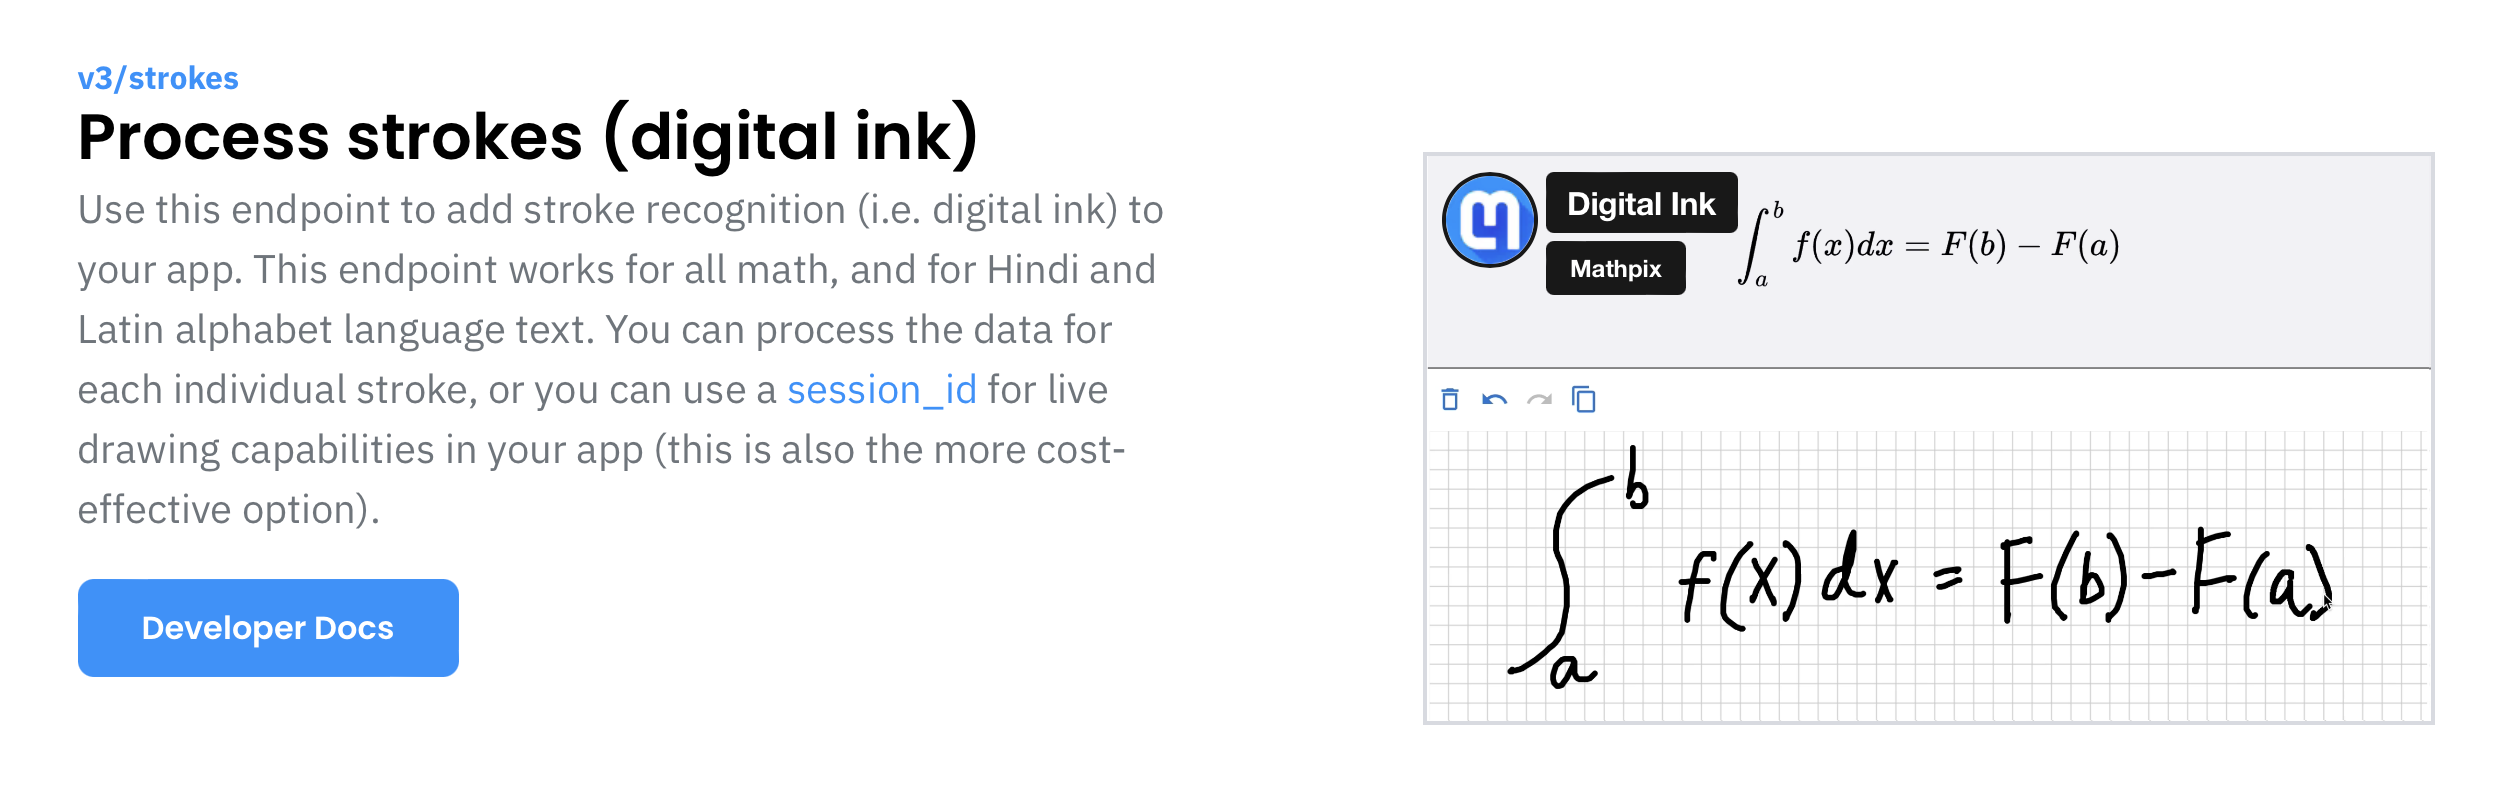
\includegraphics[width=\linewidth]{stroke_api.png}
    \caption{Mathpix 的笔迹识别 API}
    \label{fig:stroke_api}
\end{figure}

把学生的手写内容转化成文本,除了使用手写板收集到的笔迹数据,我们还可以使用 OCR 技术,把手写内容拍照或扫描成图片后将图像中的文字转化为文本。这种方法的优点是不需要额外的硬件设备,只需要一部智能手机或者平板电脑就可以实现。在手写板之外还考虑 OCR 主要有两方面原因。首先从实际落地的角度来看,手写板的采集方法需要额外的硬件设备,使用成本较高,也与我们的合作学校二十一中已有的智能教育实践不符。二十一中目前的做法是将每天的作业印在专门的答题纸上,学生作答收上来之后统一扫描,老师在电脑上查看扫描后每道题的解答区域对应的图片来阅卷。如果使用 OCR 来识别学生的手写数据的话,可以较快地融入二十一中已有的系统中。其次,与笔迹信息转文本相比,OCR 是一个更成熟的技术,效果往往更好。比如 Mathpix 的主业就是数学公式 OCR 识别,无论是使用便捷程度、灵活度还是识别效果都要优于笔迹识别。近年快速发展的多模态大语言模型如 GPT-4 Vision 等,也在图像识别领域取得了巨大的进展。因此,我们在后续的用户实验中,实际上更多使用 OCR 技术来识别学生的手写内容。

\subsection*{音频信息}

音频信息转文本我们使用飞书妙记。飞书妙记是一个在线的语音转文字服务,主要用于将会议录制音频信息转化为文本,附带时间戳信息和说话人区分。它的转文本效果比较符合我们的要求,而且可以比较好地支持较长音频文件的识别,我们将学生的音频信息上传到飞书妙记,就可以得到我们需要的文本信息。

\subsection*{视频信息}

对于视频信息,我们可以通过面部识别来观察眼动信息以及面部特征的变化。对于这个任务,可以利用Google的MediaPipe进行视频信息的实时检测和特征标定。MediaPipe是Google开发的一个较为成熟的深度学习框架,为常见的CV任务(物体探测、图像分类、手部骨架识别、人体姿态识别等)提供了训练好的模型和完善的跨平台 API (web, Android, python, iOS),效果很好。利用Mediapipe 提供的 FaceLandmark 任务实现,我们可以获取到面部网格信息以及进行面部特征提取。某一时刻的面部信息识别结果中的面部特征列表如图\ref{fig:face_features}所示。

\begin{figure}
    \centering
    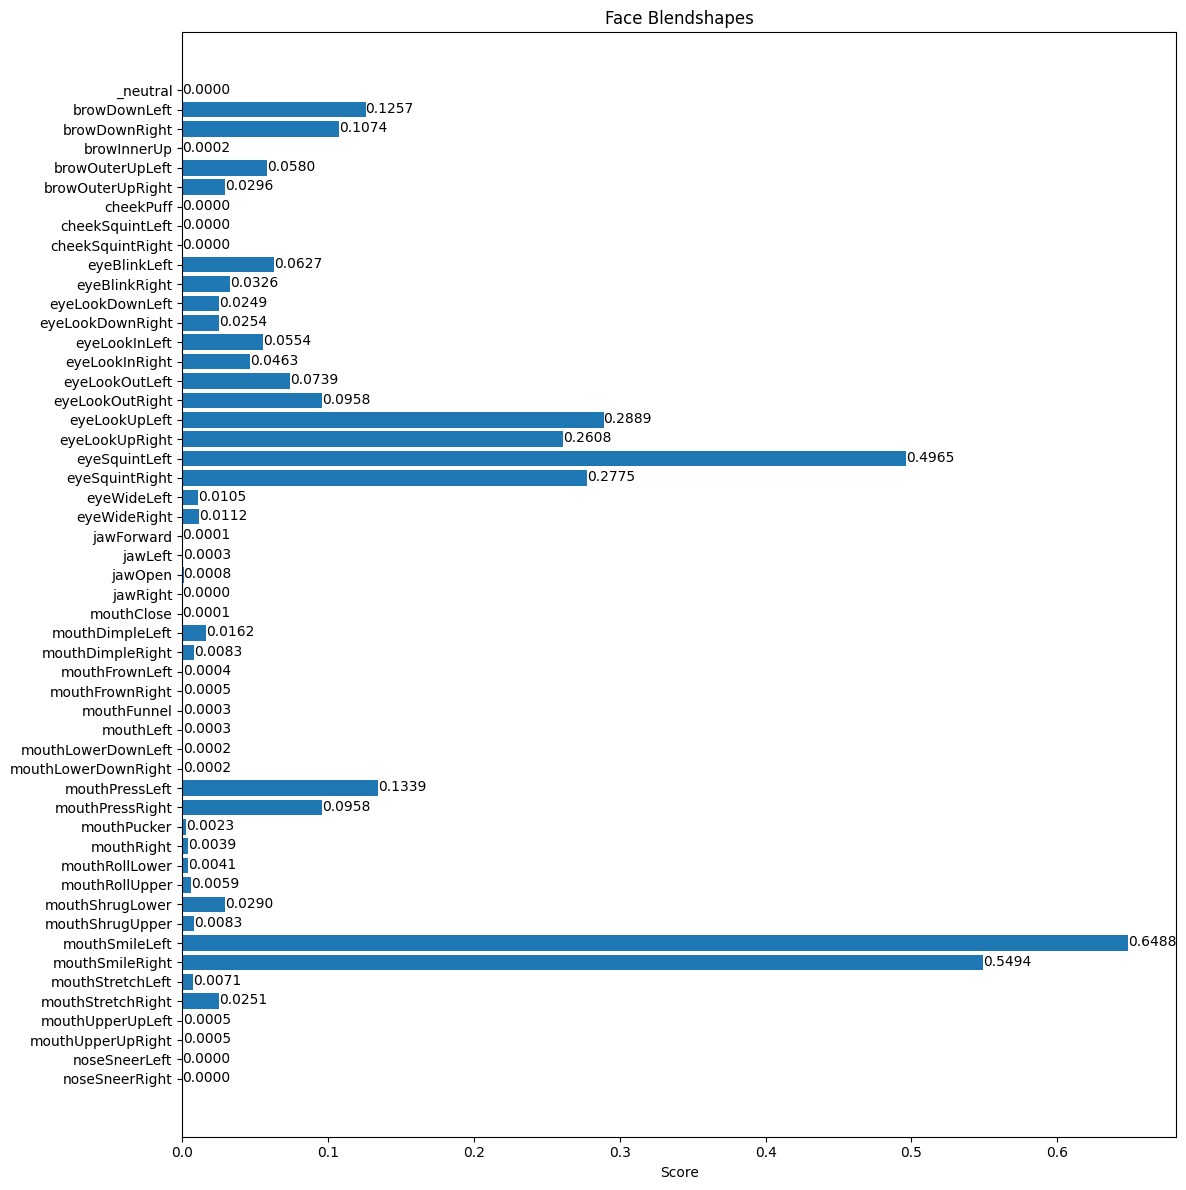
\includegraphics[width=0.7\linewidth]{face_features.png}
    \caption{Mediapipe 的面部特征识别结果示例}
    \label{fig:face_features}
\end{figure}

\section{自动批改流程}

本研究提出的解题过程评估系统的流程如图 \ref{fig:system_design} 所示。其中蓝色部分是输入,包含手写文本、语音文本和题目标准解答计算图这三部分信息;黄色背景的两个步骤是进行分析的核心步骤,由 LLM 驱动进行分析,通过调用 GPT-4 API 来进行。

\begin{figure}
    \centering
    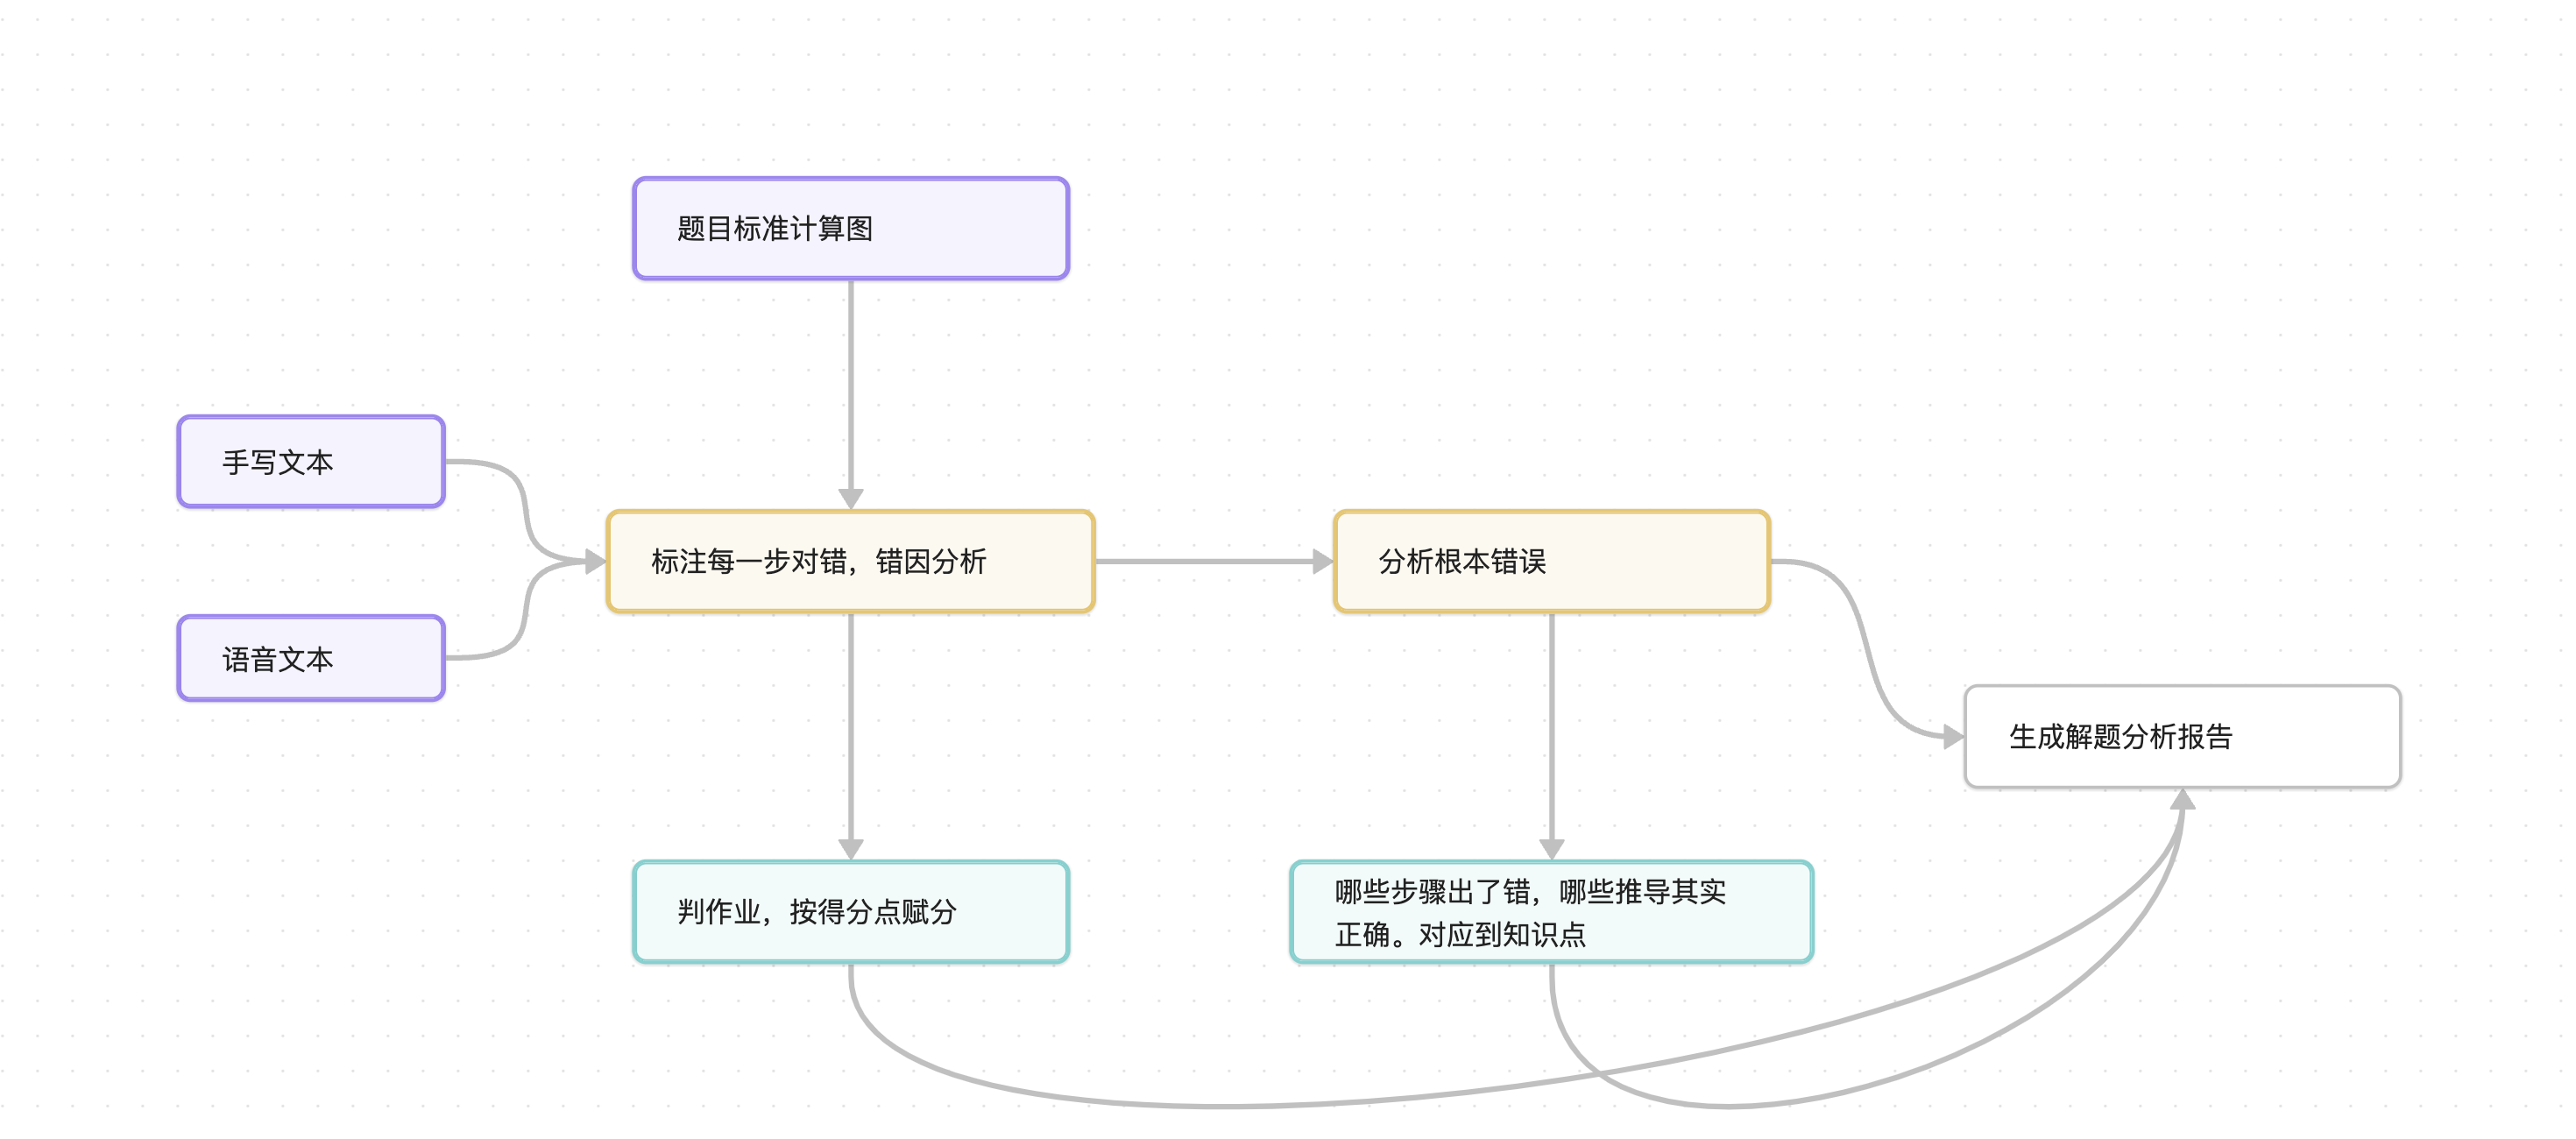
\includegraphics[width=\linewidth]{system_design.png}
    \caption{解题过程评估系统流程}
    \label{fig:system_design}
\end{figure}

\subsection*{输入}

对于一道指定的数学解答题,分析系统的输入包括学生的笔迹文本信息、解题过程 think aloud 音频转文本信息,以及这道题的标准解答计算图。笔迹和音频文本由前文所述的数据处理模块提供;标准解答计算图由人类专家进行手动标注,以 json 格式的文本输入,后续的应用上可以通过一个正确的解题过程来自动生成。

\subsection*{判断每一步的正误}

这一步的目标是对照着这道题的标准计算图分析学生的解题过程(包括语音文本和笔迹记录),标注每一步的正误情况,判断学生是否正确完成了这一步。如果学生错误,则需要给出错误原因的分析。对于每个节点正误的判断,只要学生在这一步求出了和当前节点内容结果相同或数学上等价的结果,就认为学生这一步做对了,不用关心学生具体得到这一结果的过程。具体来讲,给标准计算图中的每个节点新增一个属性 correctness (字符串),有 3 种可能取值:

\begin{itemize}
    \item correct: 学生正确完成了这一步,得到了与这步的标准结果相同或等价的结果。
    \item incorrect: 学生在这一步得到了错误的结果。
    \item unknown: 学生没有进行这一步计算或推导,可能是因为学生忘记了进行这步推导、跳过了这一步、选择了其他的解题方法等。
\end{itemize}

此外还会新增一个属性 analysis (字符串),如果 correctness 为 incorrect,这里给出错误原因的分析;如果 correctness 为 unknown,这里则是对于学生具体如何没做这步推导、缺了什么信息的说明。

\subsection*{分析根本错误点}

对于一个给定的结果不正确的节点,有两种可能。第一种情况是学生这步犯了错(知识记错了,计算错误,笔误等);第二种情况是学生这一步推导本身没错,是这步推导所依赖的前置某个节点错误导致推导结果和正确答案不符。无论这步推导依赖的节点正确与否,学生都有可能在这步犯错。这一步的任务就是分析给定节点的错误到底是这两种情况中的哪个。

在上一步正误分析的基础上,这一步分析可以找出所有学生真正出错的步骤,随后就可以针对这些出错的步骤进行错因分析,并分析学生所欠缺的能力以及没有掌握的知识有哪些。

\subsection*{生成解题分析报告}

根据上述两步分析的结果,生成解题分析报告。这一解题分析报告包括学生每一步的正误情况、学生出错的步骤的错因分析,以及学生没有掌握的知识点总结。标准图中的每一个节点都有对应的推导依赖(详见上文对计算图结构的介绍),把所有学生出错的步骤的依赖中所有知识点汇总,就是这道题涉及到的学生没有掌握的知识点。对于一个学生的解题过程,解题分析报告的例子如图\ref{fig:analysis_example}。

\begin{figure}
    \centering
    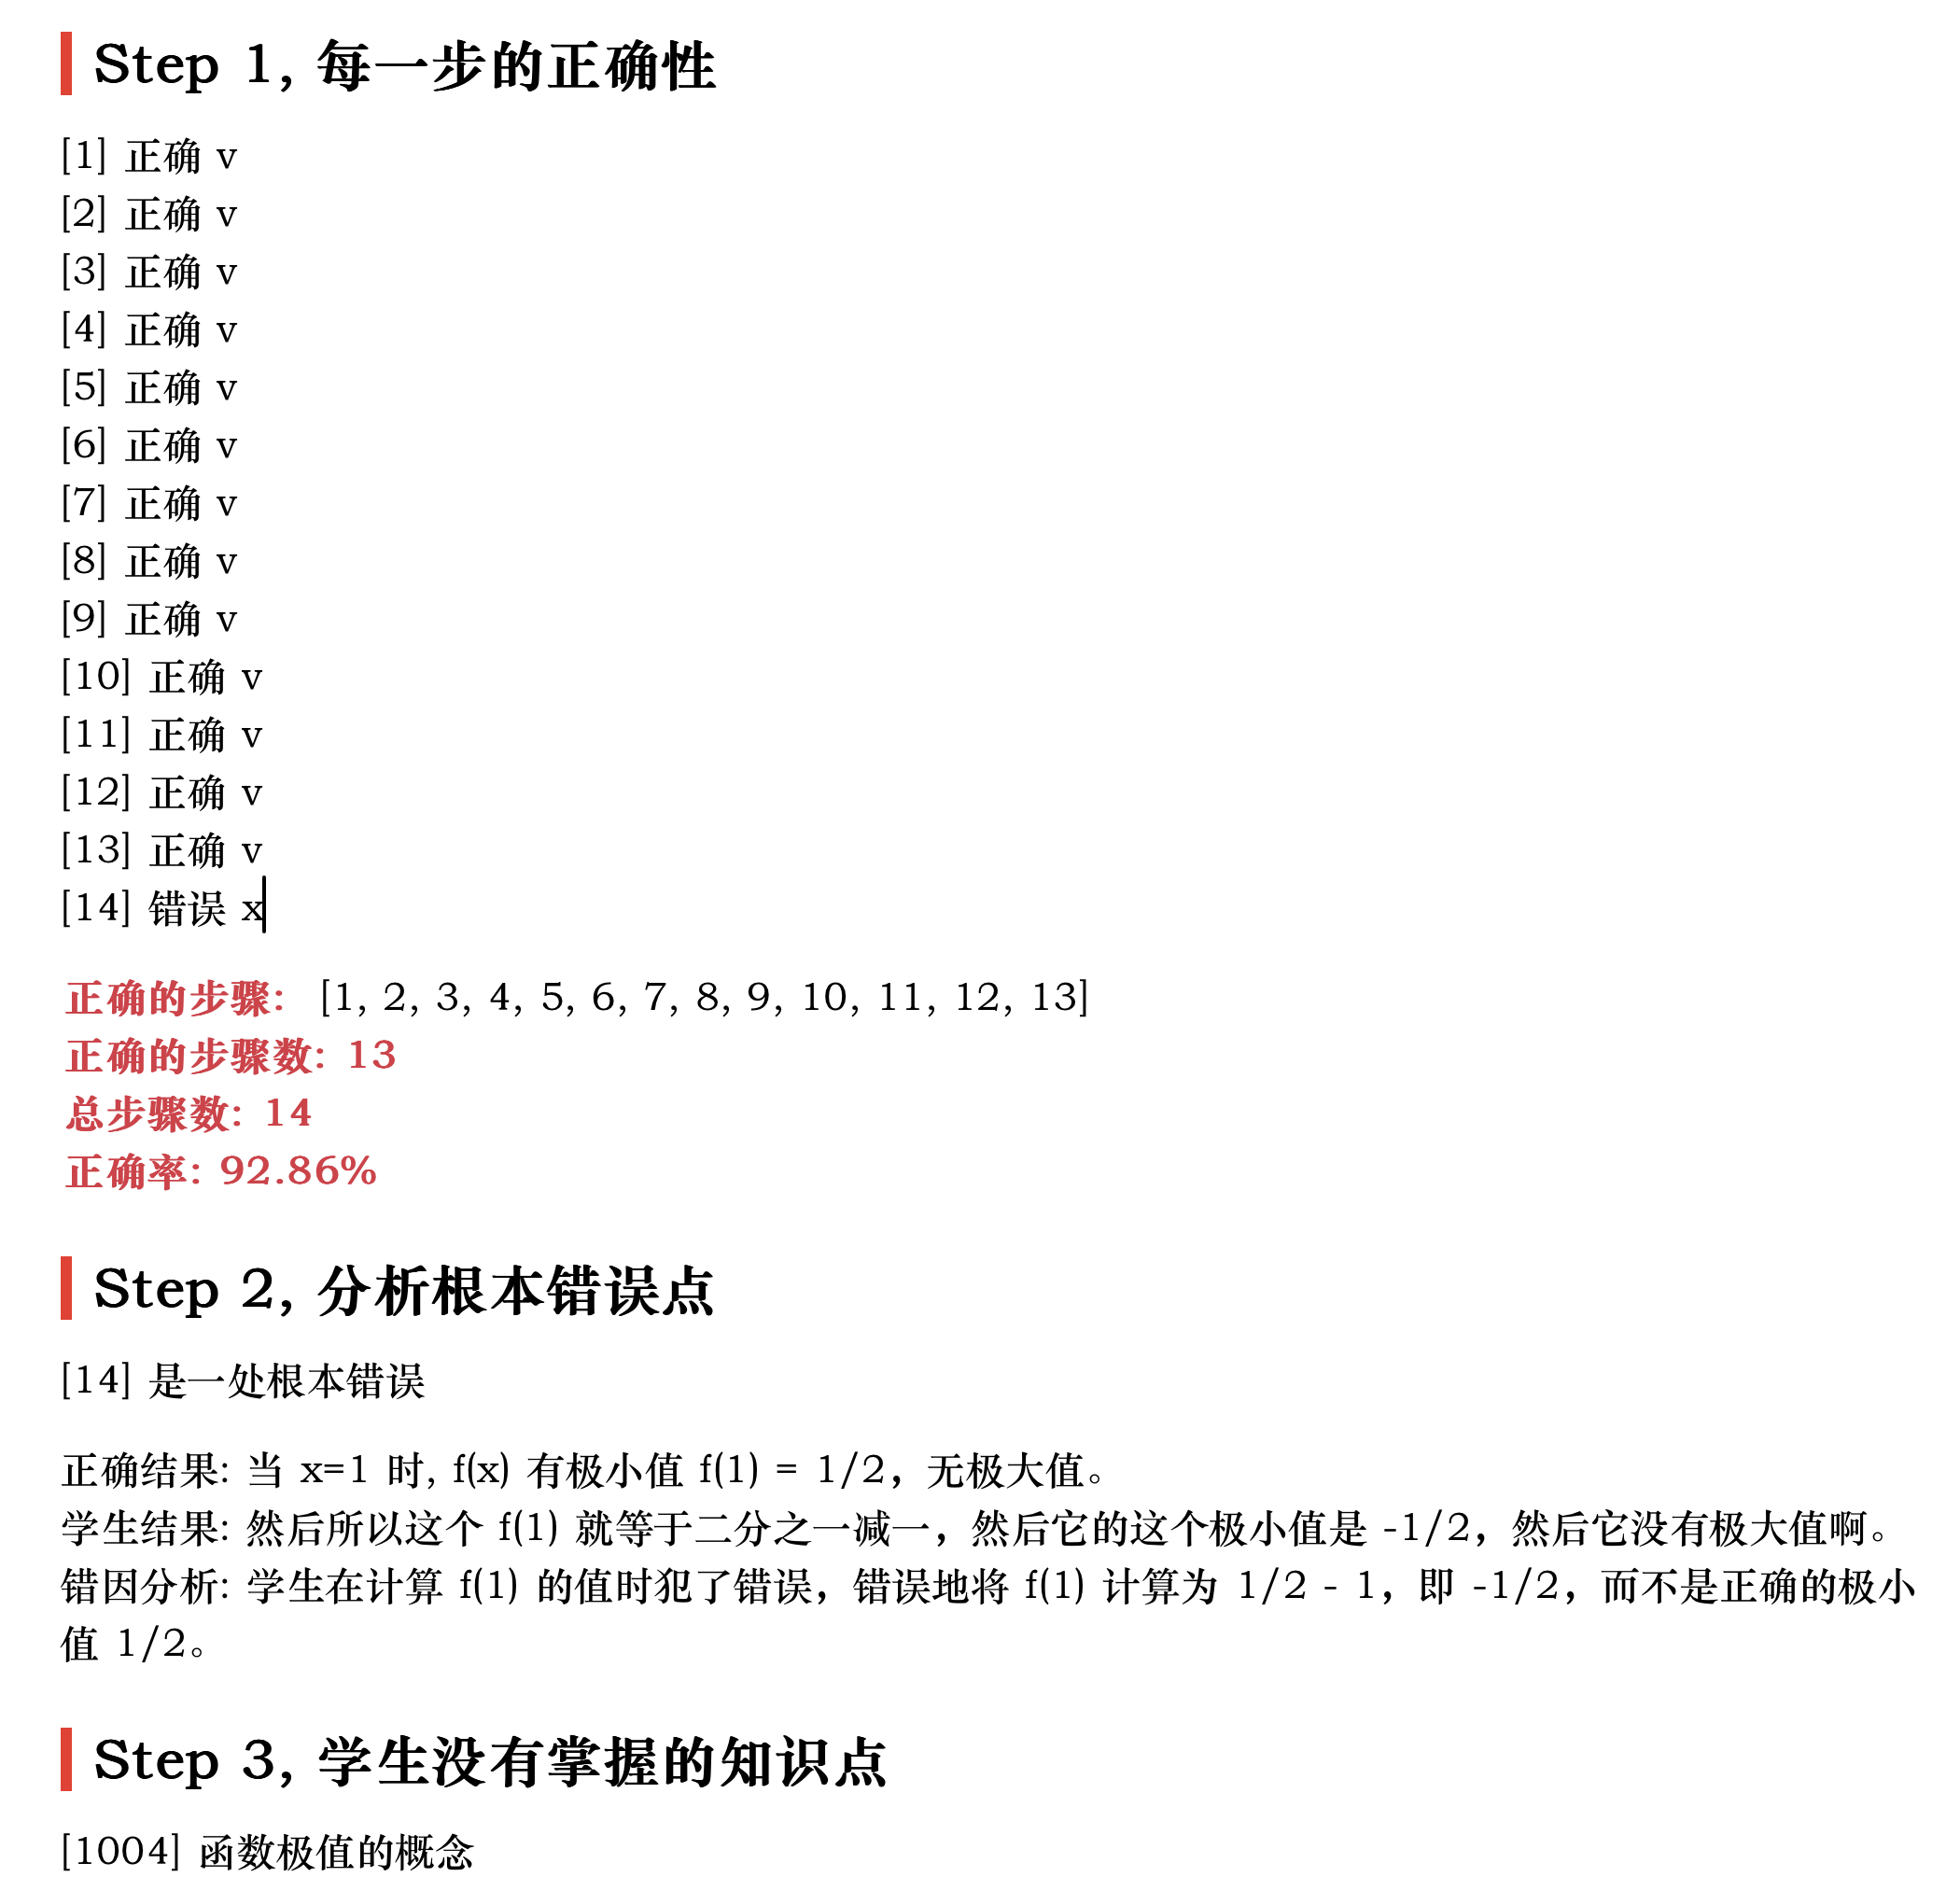
\includegraphics[width=\linewidth]{analysis_example.png}
    \caption{解题分析报告样例}
    \label{fig:analysis_example}
\end{figure}